\section{Overview of Data Enrichment Algorithm}

Our Data Enrichment Framework (DEF) takes two inputs -- 1) an instance of a data object to be enriched 
and 2) a set of data sources to use for the enrichment -- and outputs an enriched version of the input 
instance. 

DEF enriches the input instance through the following steps. DEF first assesses the importance of each 
attribute in the input instance. This information is then used by DEF to guide the selection of appropriate 
data sources to use. Finally, DEF determines the utility of the sources used, so it can adapt its usage 
of these source (either in a favorable or unfavorable manner) going forward.


\subsection{Preliminaries}

A data object $D$ is a collection of attributes describing a real-world object of interest. We formally
define $D$ as $\lbrace a_1, a_2, ... a_n \rbrace$ where $a_i$ is an attribute.

An instance $d$ of a data object $D$ is a partial instantiation of $D$ -- i.e. some attributes $a_i$ may 
not have an instantiated value. We formally define $d$ as having two elements $d_k$ and $d_u$. $d_k$ 
consists of attributes whose values are known (i.e. instantiated), which we define formally as $d_k = 
\lbrace <a,v(a),k_a,k_{v(a)}> ... \rbrace$, where $v(a)$ is the value of attribute $a$, $k_a$ is the 
importance of $a$ to the data object $D$ that $d$ is an instance of (ranging from 0.0 to 1.0), and 
$k_{v(a)}$ is the confidence in the correctness of $v(a)$ (ranging from 0.0 to 1.0). $d_u$ consists of 
attributes whose values are unknown and hence the targets for enrichment. We define $d_u$ formally as 
$d_u= \lbrace <a,k_a> ... \rbrace$.

\subsection{Attribute Importance Assessment} 

Given an instance $d$ of a data object, DEF first assesses (and sets) the importance $k_a$ of each 
attribute $a$ to the data object that $d$ is an instance of. DEF uses the importance to guide the 
subsequent selection of appropriate data sources for enrichment (see next subsection).

Our definition of importance is based on the intuition that an attribute $a$ has high importance to a data object
$D$ if its values are highly unique across all instances of $D$. For example, the attribute {\it e-mail contact} 
should have high importance to the {\it Customer} data object because it satisfies this intuition. However, 
the attribute {\it Zip} should have lower importance to the {\it Customer} object because it does not -- i.e. 
many instances of the {\it Customer} object have the same zipcode.

DEF captures the above intuition formally with the following equation:
\begin{equation}
	k_a= \sqrt{\frac{X^2}{1+ X^2}}
\end{equation}
where, 
\begin{equation}
	X = H_{N(D)}(a) \left(\frac{U(a,D)}{|N(D)|}\right)
\end{equation}
and
\begin{equation}
	H_{N(D)}(a)= - \displaystyle\sum\limits_{v \in a} P_v log P_v
\end{equation}
$U(a,D)$ is the number of unique values of $a$ across all instance of the data object $D$ observed by 
DEF so far, and $N(D)$ is all instances of $D$ observed by DEF so far. $H_{N(D)}(a)$ is the entropy of 
the values of $a$ across $N(D)$, and serves as a proxy for the distribution of the values of $a$. 

We note that DEF recomputes $k_a$ as new instances of the data object containing $a$ are observed. Hence, 
the importance of an attribute to a data object will change over time.


\subsection{Data Source Selection} 

DEF selects data sources to enrich attributes of a data object instance $d$ whose values are unknown. 
DEF will repeat this step until either there are no attributes in $d$ whose values are unknown or there 
are no more sources to select.

DEF considers two important factors when selecting the next best source to use: 1) whether the source will 
be able to provide values if called, and 2) whether the source targets unknown attributes in $d_u$ (esp.
attributes with high importance). DEF satisfies the first factor by measuring how well known values of $d$ 
match the inputs required by the source. If there is a good match, then the source is more likely to return 
values when it's called. DEF also considers the number of times a source was called previously (while enriching 
$d$) to prevent ``starvation" of other sources. 

DEF satisfies the second factor by measuring how many high-importance, unknown attributes the source claims 
to provide. If a source claims to provide a large number of these attributes, then DEF should select the 
source over others. This second factor serves as the selection bias. 

DEF formally captures these two considerations with the following equation:
\begin{equation}
    F_s = \frac{1}{2^{M-1}}B_s \frac{\displaystyle\sum\limits_{a \in d_k \cap I_s} k_{v(a)}}{|I_s|} 
    	+ \frac{\displaystyle\sum\limits_{a \in d_u \cap O_s} k_{a}}{|d_u|}
\end{equation}
where $B_s$ is the base fitness score of a data source $s$ being considered (this value is randomly set between 
0.5 and 0.75 when DEF is initialized), $I_s$ is the set of input attributes to the data source, $O_s$ is 
the set of output attributes from the data source, and $M$ is the number of times the data source has been 
selected in the context of enriching the current data object instance.

The data source with the highest score $F_s$ that also exceeds a predefined minimum threshold $R$ is selected
as the next source to use for enrichment.

For each unknown attribute $a'$ enriched by the selected data source, DEF moves it from $d_u$ to $d_k$, and 
computes the confidence $k_{v(a')}$ in the value provided for $a'$ by the selected source. This confidence 
is used in subsequent iterations of the enrichment process, and is computed using the following formula: 
\begin{equation}
 \label{_output_confidence}
	k_{v(a')} = \left\lbrace 
		\begin{array}{ll}
			e^{ \left( \frac{1}{|V_{a'}|} - 1 \right) } W \nonumber & \mbox{, if } k_{v(a')} = Null \\
			e^{\lambda(k_{v(a')} - 1)} 				& \mbox{, if } k_{v(a')} \neq Null \\
		\end{array}
		\right.
\end{equation}
where,  
\begin{equation}
	W = \frac{\displaystyle\sum\limits_{a \in d_k \cap I_s} k_{v(a)} }{|I_s|}
\end{equation}
$W$ is the confidence over all input attributes to the source, and $V_{a'}$ is the set of output values 
returned by a data source for an unknown attribute $a'$. 

This formula captures two important factors. First, if multiple values are returned, then there is ambiguity 
and hence the confidence in the output should be discounted. Second, if an output value is corroborated 
by output values given by previously selected data sources, then the confidence should be further increased. 
The $\lambda$ factor is the corroboration factor ($< 1.0$), and defaults to 1.0.

In addition to selecting appropriate data sources to use, DEF must also resolve ambiguities that occur 
during the enrichment process. For example, given the following instance of the {\it Customer} data object:
\begin{quote}
	(Name: John Smith, City: San Jose, Occupation: NULL)
\end{quote}
a data source may return multiple values for the unknown attribute of {\it Occupation} (e.g. Programmer, 
Artist, etc).

To resolve this ambiguity, DEF will branch the original instance -- one branch for each returned value -- 
and each branched instance will be subsequently enriched using the same steps above. Hence, a single data 
object instance may result in multiple instances at the end of the enrichment process. 

DEF will repeat the above process until either $d_u$ is empty or there are no sources whose score 
$F_s$ exceeds $R$. Once this process terminates, DEF computes the fitness for each resulting instance 
using the following equation:
\begin{equation}
	\frac{\displaystyle\sum\limits_{a \in d_k \cap d_U} k_{v(a)} k_a }{|d_k \cup d_u|}
\end{equation}
and returns top $K$ instances.


\subsection{Data Source Utility Adaptation}

Once a data source has been called, DEF determines the utility of the source in enriching the data
object instance of interest. Intuitively, DEF models the utility of a data source as a ``contract" 
-- i.e. if DEF provides a data source with high confidence input values, then it is reasonable to 
expect the data source to provide values for all the output attributes that it claims to target. 
Moreover, these values should not be generic and should have low ambiguity. If these expectations 
are violated, then the data source should be penalized heavily. 

On the other hand, if DEF did not provide a data source with good inputs, then the source should
be penalized minimally (if at all) if it fails to provide any useful outputs.

Alternatively, if a data source is able to provide unambiguous values for unknown attributes in 
the data object instance (esp. high importance attributes), then DEF should reward the source
and give it more preference going forward.

DEF captures this notion formally with the following equation:
%
% \begin{eqnarray}
% U_s &=& W \left( \frac{1}{|O_s|} \left( \displaystyle\sum\limits_{a \in O_s^+} e^{\frac{1}{|V_a|} - 1}k_a^{P_Tv(a)} - \displaystyle\sum\limits_{a \in 
% O_s^-}k_a \right) \right) \nonumber \mbox{ where,}\\
% P_T(v(a)) &=& \left\lbrace \begin{array}{ll} P_T (v(a)) & \mbox{, if } |V_a|= 1 \\ \argmin\limits_{v(a) \in V_a} P_T(v(a)) & \mbox{, if } |V_a| > 1 
% \end{array} \right.
% \end{eqnarray}
%
\begin{equation}
	U_s = W \left( \frac{1}{|O_s|} \left( \displaystyle\sum\limits_{a \in O_s^+} e^{\frac{1}{|V_a|} - 1}k_a^{P_Tv(a)} - \displaystyle\sum\limits_{a \in O_s^-}k_a \right) \right) \nonumber
\end{equation}
where,
\begin{eqnarray}
	P_T(v(a)) &=& \left\lbrace \begin{array}{ll} P_T (v(a)) & \mbox{, if } |V_a|= 1 \\ \argmin\limits_{v(a) \in V_a} P_T(v(a)) & \mbox{, if } |V_a| > 1 \end{array} \right.
\end{eqnarray}
$O_s^+$ are the output attributes from a data source for which values were returned, $O_s^-$ 
are the output attributes from the same source for which values were not returned, and $P_T(v(a))$
is the relative frequency of the value $v(a)$ over the past $T$ values returned by the data source for 
the attribute $a$. $W$ is the confidence over all input attributes to the source, and is defined
in the previous subsection.

The utility of a data source $U_s$ from the past $n$ calls are then used to adjust the base fitness score 
of the data source. This adjustment is captured with the following equation
\begin{equation}
 B_s= B_s + \gamma \frac{1}{n} \displaystyle\sum\limits_{1}^{n}U_s(T - i)
\end{equation}
where $B_s$ is the base fitness score of a data source $s$, $U_s(T-i)$ is the utility of the data source $i$ time steps
back, and $\gamma$ is the adjustment rate.

%
% \subsection{System Architecture}
% \begin{itemize}
%	\item Key components: modules for computing each of the attributes, RESTful integration with user interface, Comet pattern, APIs
%	\item Underlying technologies: Django, jQuery, celery
% \end{itemize}
%
%
\section{System Architecture}

\begin{figure}[htb]
\centering
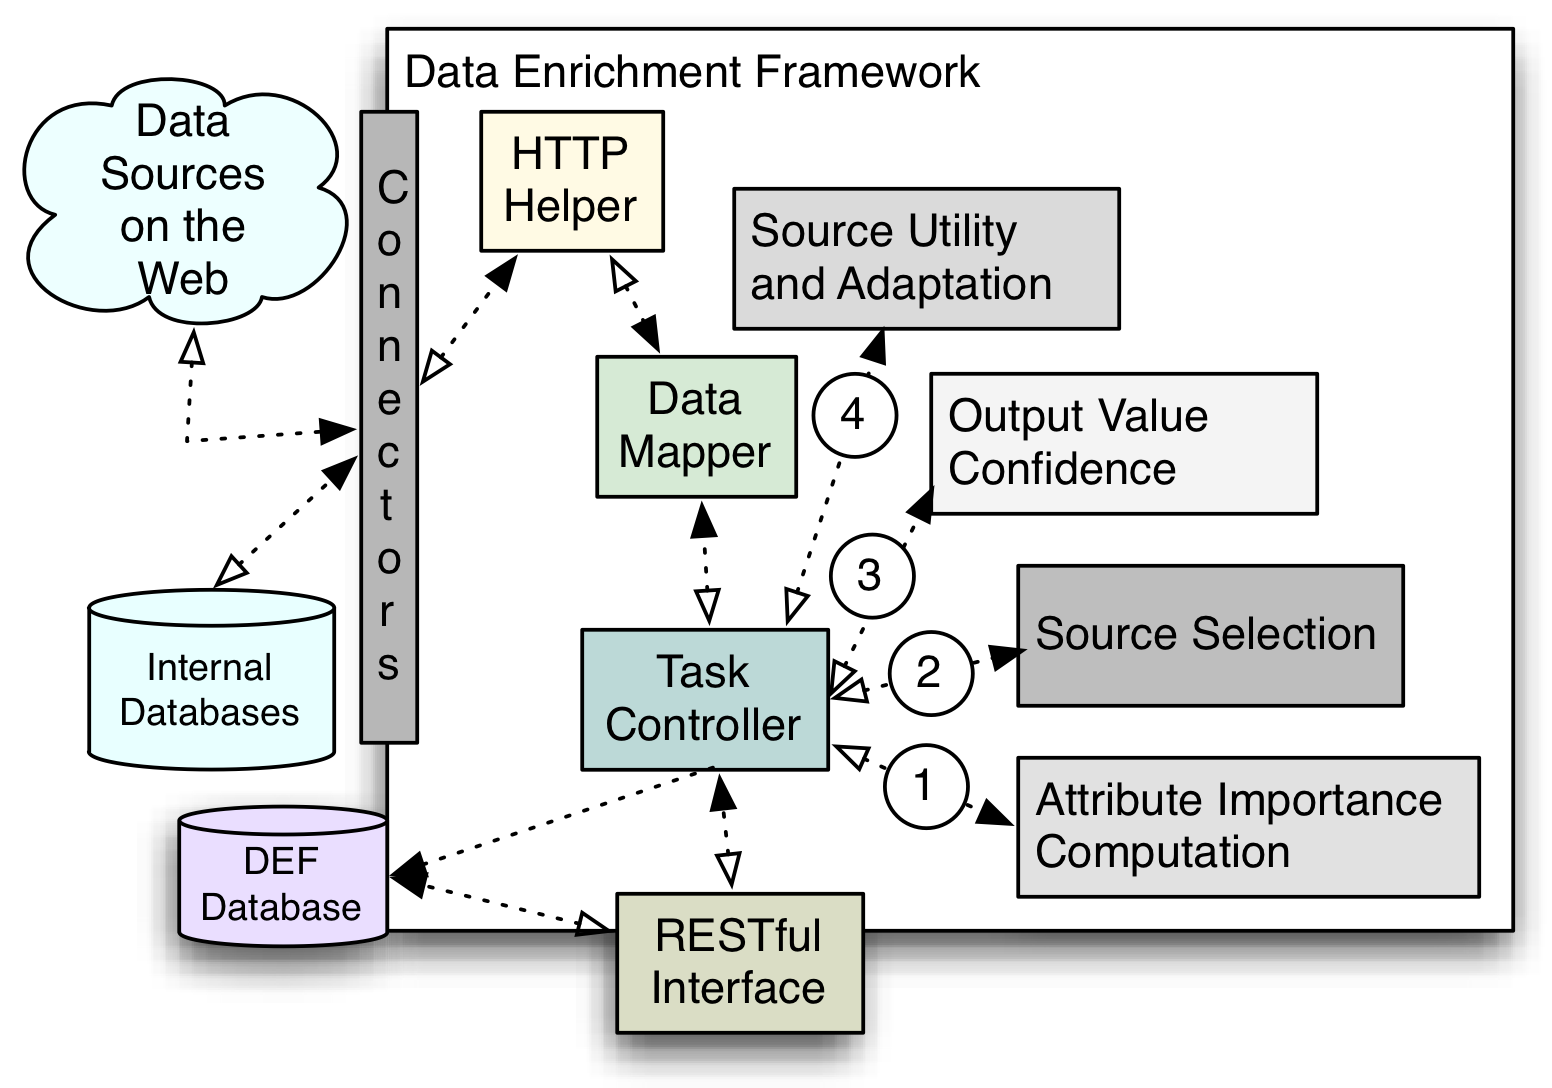
\includegraphics[width=0.45\textwidth]{images/adef_arch.png}
\caption{Design overview of enrichment framework}
\label{fig:overview}
\end{figure}

The main components of DEF are illustrated in Figure \ref{fig:overview}. The task manager starts a new enrichment project by instantiates and executes the enrichment engine.
The enrichment engine uses the attribute computation module to calculate the attribute relevance. The relevance scores are used in source selection. Using the HTTP helper module, the engine then invokes 
the connector for the selected data source. A connector is a proxy that communicates with the actual data source and is a RESTful Web service in itself. The enrichment framework requires every data source to have a connector and 
that each connector have two operations: 1) a return\_schema GET operation that returns the input and output schema, and 2) a get\_data POST operation that takes as input the input for the data source as POST parameters and returns 
the response as a JSON. For internal databases, we have special connectors that wrap queries as RESTful end points. 
Once a response is obtained from the connector, the enrichment engine computes the output value confidence, applies the necessary mapping rules, and integrates the response with the existing data object. In 
addition to this, the source utility is also computed. The mapping, invocation, confidence and source utility value computation steps are repeated until either all values for all attributes are computed or if all sources
have been invoked. The result is then written into the enrichment database.  

In designing the enrichment framework, we have adopted a service oriented approach, with the goal of exposing the enrichment framework as a ``platform as a service''. 
The core tasks in the framework are exposed as RESTful end points. These include end points for 
creating data objects, importing datasets, adding data sources, and for starting an enrichment task. When the ``start enrichment task'' task resource is invoked and a task is successfully started, the framework responds with a JSON 
that has the enrichment task identifier. This identifier can then be used to GET the enriched data from the database. The framework supports both batch GET and streaming GET using the comet \cite{comet} pattern. 

Data mapping is one of the key challenges in any data integration system. While extensive research literature exists for automated and semi-automated approaches for mapping and matching \cite{mapping1,mapping2}
it is our observation that these techniques do not guarantee the high-level of accuracy required in enterprise solutions. So, we currently adopt a manual approach, aided by a graphical interface for data mapping. The source and 
the target schemas are shown to the users as two trees, one to the left and one to the right. Users can select the attributes from the source schema and draw a line between them and attributes of the target schema. Currently, our
mapping system supports assignment, merge, split, numerical operations, and unit conversions. When the user saves the mappings, the maps are stored as mapping rules. Each mapping rule is represented as a tuple containing the 
source attributes, target attributes, mapping operations, and conditions. Conditions include merge and split delimiters and conversion factors.  
